\documentclass{article}
\usepackage[utf8]{inputenc}
\usepackage{graphicx}
	\DeclareGraphicsExtensions{.png, .jpeg}
\usepackage[top=1in, bottom=1in, left=1in, right=1in]{geometry}
\usepackage[named]{algo}

\title{Autonomoboro \\ Lab06: Ball Sorting}
\author{Bandith Phommounivong, Terence Henriod}
\date{\today}

\begin{document}

\maketitle

\begin{abstract}
A discussion of the design and performance of a robot designed to dump balls over certain sides of a table depending on their color.
\end{abstract}

\newpage
\section{Robot Design}
A robot design that was capable of carrying a lot of hardware was chosen, for better or for worse. The design featured almost every item in the given NXT kit and utilized nearly every sensor at one point in it's programming or another. The design also featured a large claw that trapped balls very well, and its software controller was designed to be very methodical and procedurally driven.

\subsection{Hardware Configuration}
The ball sorting competition demanded an entirely new level of design and hardware feature breadth. The design required the robot to not only be able to localize itself and move in some sort of desirable pattern, but the robot needed to be able to detect and manipulate objects in a 3-dimensional environment. This resulted in what might be termed ``hardware bloat," but the robot was still sufficiently functional. The robot featured six sensors, a large trapping claw and some trapping arms, a multiplexer, a tall compass tower, and a large ball for a caster wheel.

\subsubsection{Chassis}
The chassis of the robot was a tightly constructed 3-motor chassis with 2 driving wheels and a passive caster ``wheel". The motors were grouped tightly together, and the NXT brick sat atop the motor cluster. Extending to the rear was a cage to hold the caster ``wheel" that supported a small platform for holding the multiplexer and its battery pack. Extending to the front of the robot were a pair of arms and a large trapping claw/cage. Attached to the side of the robot and extending upward was a compass tower for holding the compass sensor.

	\begin{figure}[h]
	\centering
	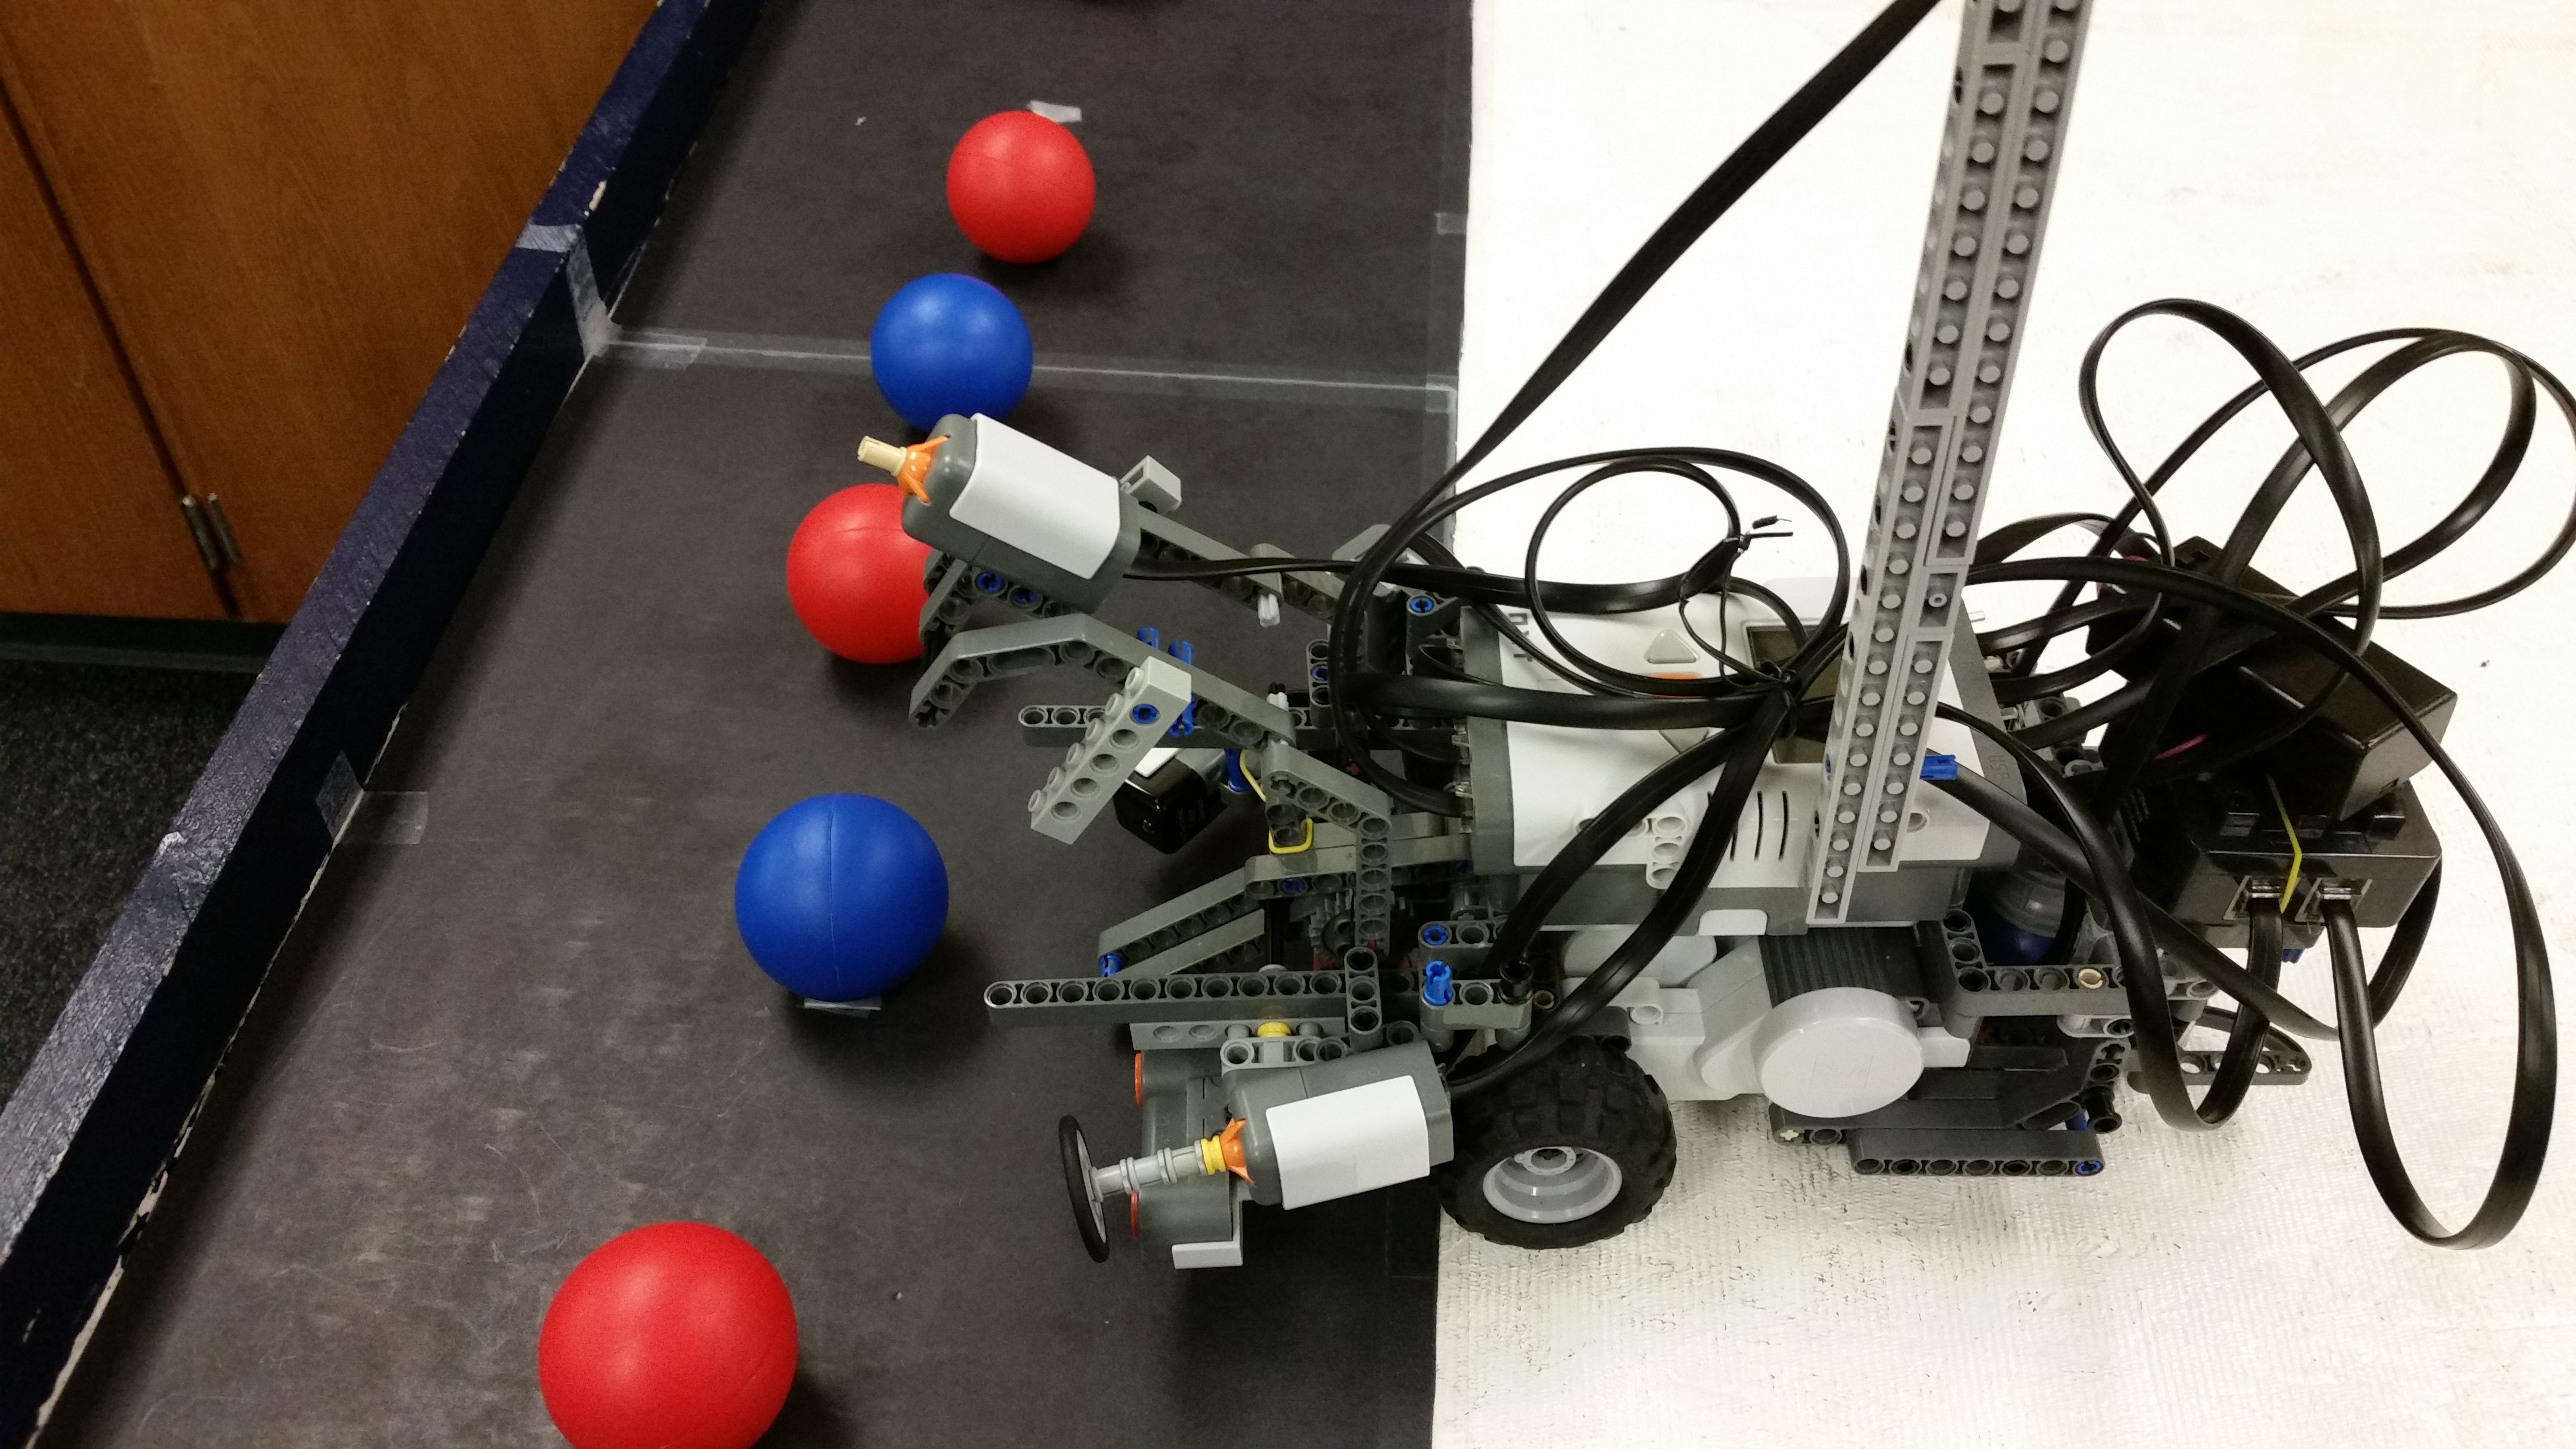
\includegraphics[width = 0.4\textwidth]{side_view}
        % extension usually unnecessary when specifying file
	\caption{A side view of the robot}
	\label{fig:side_view}
	\end{figure}

\begin{description}
  \item[Caster Ball] \hfill \\
  The caster ball (in place of a wheel) was an NXT competition ball and functioned surprisingly well. It provided excellent load bearing capacity and relatively high mobility. The load bearing capacity was greatly desired since the weight of the multiplexer and any apparatus securing it would cause other caster wheel solutions to bow out and risk ruining the lego parts. Due to the smoothness of the arena floor and the ball, the ball would glide easily over the floor.

  \item[Ball Trapping Apparatus] \hfill \\
  This apparatus required intricate design, due to the fact that it had to be made out of a scant assortment of parts along with the fact that there was a large degree of functionality it needed to support. The main feature of the apparatus was the cage claw that could be raised and lowered to trap or release a ball. On the front of the claw, there was a bump sensor for detecting when the claw should be raised. Assisting the claw (although, probably more valuable) were two arms protruding from the robot. The arms were set at a height just above the arena walls so that the robot could drive right up to the wall without relinquishing control of the ball. The arms also supported two sensors each, which were both useful for sensing, as well as further trapping the ball. Inside the trapping apparatus was a short, steep ramp and a small extension situated at the top of the ramp. These were used to push balls up and over the wall of the arena when the robot drove forward with the claw raised.

  \item[Compass Tower] \hfill \\
  The compass tower was built to be tall and showy. While the compass sensor did need to be held away from the other electronics, this height was excessive. Excessive to demonstrate authority.
\end{description}


\subsubsection{Sensors}
Six sensors in total were used: a color sensor, a compass sensor, a light/reflectance sensor, a sonar sensor, and two bump sensors.

\begin{description}
  \item[Color Sensor] \hfill \\
  The color sensor was fixed under the left arm and pointed at a heading just in front of the ramp. It was used to detect when a ball had been brought inside trapping range for the robot.

  \item[Compass Sensor] \hfill \\
  The compass sensor was arguably one of the more valuable sensors. It was placed high up on the compass tower and was used for orienting the robot. The sensor was not high integrity, much like any other NXT sensor, but it was useful enough.

  \item[Reflectance Sensor] \hfill \\
  The reflectance sensor was attached just above and outside of the right arm. This sensor was essential for localization at the ball dumping ends of the arena. These ends were marked with a black floor. Reflectance was essential for localization since the sonar might be fooled by balls that remained in the end zones.

  \item[Sonar Sensor] \hfill \\
  The sonar sensor was used to detect walls that were not part of the end zones. This allowed the robot to drive up to those walls to help position itself when lining up to capture balls. This sensor was arguably extraneous (it could have been replaced with bump sensing), but it was included in the hopes that it could enhance robot localization. The sensor was attached under the left arm to allow it to sense walls.

  \item[Touch Sensor One] \hfill \\
  The first bump sensor was attached to the front of the trapper claw. Since the claw was only lowered when a ball was in tow, this sensor could be used to detect when the robot had reached a wall that a ball should be dumped over.

  \item[Touch Sensor Two] \hfill \\
  A second touch sensor was added in the hopes of providing additional functionality to the robot once all of the balls had been knocked away from their starting positions.The sensor was fixed on the left side, just above the sonar sensor. It featured a protruding rod with a wheel on the end to help it reach out and contact a wall should the ball robot not encounter any balls when seeking them. Unfortunately, it was decided that since the competition time was so short, it was decided to not implement additional strategies, effectively rendering this sensor a kill switch/button.
\end{description}

\newpage
\subsection{Software Design}
The software design was modular and relatively simple. It featured a driver/controller with an action sequence composed of just a few general actions: find the corner of the ball area to start, creep up to and capture a ball, and dump the ball over the appropriate edge. Supporting the controller was a publish-subscribe architecture for the sensing capabilities.

\subsubsection{Overall Algorithm}
The psuedo-code for the control algorithm is as follows: \\
\begin{algorithm}{SORT-BALLS}[]{
  \qwhile Time Remaining $\neq 0$ \\
  \qdo \\
    Drive to East wall \\
    Drive to the South wall \\
    Turn to the West \\
    \qrepeat \\
      Creep Southward \\
    \quntil Ball detected \\
    Capture ball \\
    \qif $Ball.color \eq red$ \\
      \qthen Dump the ball at the South end of the arena \\
      \qelse \qif $Ball.color \eq blue$ \\
        \qthen Dump the ball at the North end of the arena \\
      \qfi \\
    \qfi \\
    Back out into the middle of the arena \\
  \qelihw
\end{algorithm}

\begin{description}
  \item[Guiding Walls] \hfill \\
  The robot used the walls to help situate itself in the ball area. By driving to the East wall, the robot was able to start at one end of the ball area. Then the robot drove into the black area, completing its transition to the ball area. Finally, a series of small movements were executed to properly align the robot for ball capturing. The compass sensor was essential to determining which walls to drive to.

  \item[Creep and Capture] \hfill \\
  Once the robot was ready to search for balls, it simply drove forward at a slow pace so as not to unnecessarily disrupt the balls. Once the color sensor found a reading of either ball color, the robot immediately dropped the claw to trap the ball. Once a ball was captured, the robot would back up a little to avoid uncaptured balls and prepare for ball dumping.

  \item[Ball Dumping] \hfill \\
  The strategy was simple: drive to the appropriate area to dump a ball, drive until the robot hit the wall to be dumped over, back up just a little, raise the claw, then drive forward quickly to push the ball up the robot's ramp and punch it over the wall with the robot's ball-punching extension. This was a consistent operation as long as the robot was properly oriented.
\end{description}

\subsubsection{Publish-Subscribe Architecture}
As it was with previous designs, a publish-subscribe model was used. That is to say, each sensor and the controlling logic ran in their own threads. Sensor readings were ``published" by storing their data in sensor-data-typed structs. The controller thread ``subscribed" to the data by polling the structs as appropriate. The sensor threads could have their readings turned on or off as needed, ideally in order to save on CPU time, power, etc.

\newpage
\section{Issues with the Robot}
In summary, issues pertaining to the robot were more complex than in previous competitions, and were solved simply through creativity and dedication.

\subsection{Implementation Problems and Their Solutions}
The problems that arose during the development of the ball-sorting robot were subtle and often tricky to resolve.

\begin{description}
  \item[Getting Close to the Wall During Ball Dump] \hfill \\
  It was difficult creating the right combination and arrangement of parts to enable the successful ball dump: the guide arms needed to be high enough to pass over the wall, the sensors attached on the arms needed to sit far enough back to allow the robot to get close to the wall, the ramp and extension needed to be set at just the right angles and distances, and so on. This was solved through perseverance, creativity, and trying many arrangements of things until an acceptable one was found.

  \item[Buggy Sensors] \hfill \\
  As per the usual, the sensors were relatively unreliable. The resolution to this issue was to simply be more judicious in the use of each sensor, i.e. use it in ideal situations for the sensor, as well as adjust the robot control to allow for relaxed ranges of sensor readings that were indicative of significant events.

  \item[Overloaded Design] \hfill \\
  Because the design of the robot supported so many features/sensors/capabiliities, some interesting solutions needed to be implemented. Load bearing was certainly an issue, adeptly solved with the ``caster ball" solution. Many sensors needed to be attached in specific ways, giving rise to several creative attachment strategies. In short, the solution to this overloading problem was to expose as many attachment areas as possible on the robot via a bulky chassis.
\end{description}

\subsection{Unsolved Problems}
The problems that remained unsolved were either difficult to solve or very rare, but they were significant nonetheless.

\begin{description}
  \item[Buggy and Incomplete Software] \hfill \\
  Software bugs were the bane of the robot's existence. On the competition run, bugs there were bugs that caused the robot to not be controlled precisely enough, ruining its performance. One such bug caused the robot to hit a wall at a bad angle and cause it to dump a ball over a side wall and then hit the aforementioned ``kill button." This led to the performance being awarded only mercy points. More elaborate control strategies would have solved this issue. This performance was not the norm, however, since on a second ``just-to-show-I-can" run, the robot performed quite well, actually tying the the score that took first place. But alas, consistency is often preferable to occasional grand performances.

  The software might also be considered incomplete. This was because it was sufficiently complete given that the time limit seemed to be too short to merit additional strategies or because bugs presented themselves so infrequently to merit patching. Of course was shown to not be the case at the competition, and the only solution would be more time investment and testing.  


  \item[Bulkiness] \hfill \\
  The robot was bulky. It made it a little difficult to maneuver and caused it to unnecessarily scatter balls. However, the designer was proud of the robot and figured that change was not merited given the limited ball sorting time. However, it became apparent at the competition that knocking away red balls unnecessarily inhibited high score achievement. This would be a difficult problem to solve without doing a complete redesign of large components of the robot. 
\end{description}

\end{document}
